\section{Техническое задание}
\subsection{Основание для разработки}

Основанием для разработки является задание на курсовую работу "<Разработка компьютерной игры в жанре платформер на языке Python">.

\subsection{Цель и назначение разработки}

Основной целью курсовой работы является разработка компьютерной игры в жанре платформер.

Назначение проекта заключается в развлечении потенциального потребителя.

Задачами данной разработки являются:
\begin{itemize}
\item разработка архитектуры приложения;
\item разработка интерфейса приложения;
\item реализация базовой логики и физики игры;
\item создание системы конструктора уровней;
\item обработка событий;
\item реализация отображения игры на экране.
\end{itemize}

\subsection{Требования пользователя к интерфейсу игры}

Игра должна включать в себя:
\begin{itemize}
    \item возможность управления персонажем;
    \item графическое оформление интерфейса;
    \item базовый редактор уровней.
\end{itemize}

Композиция шаблона сайта представлена на рисунке ~\ref{templ:image}.

\begin{figure}[ht]
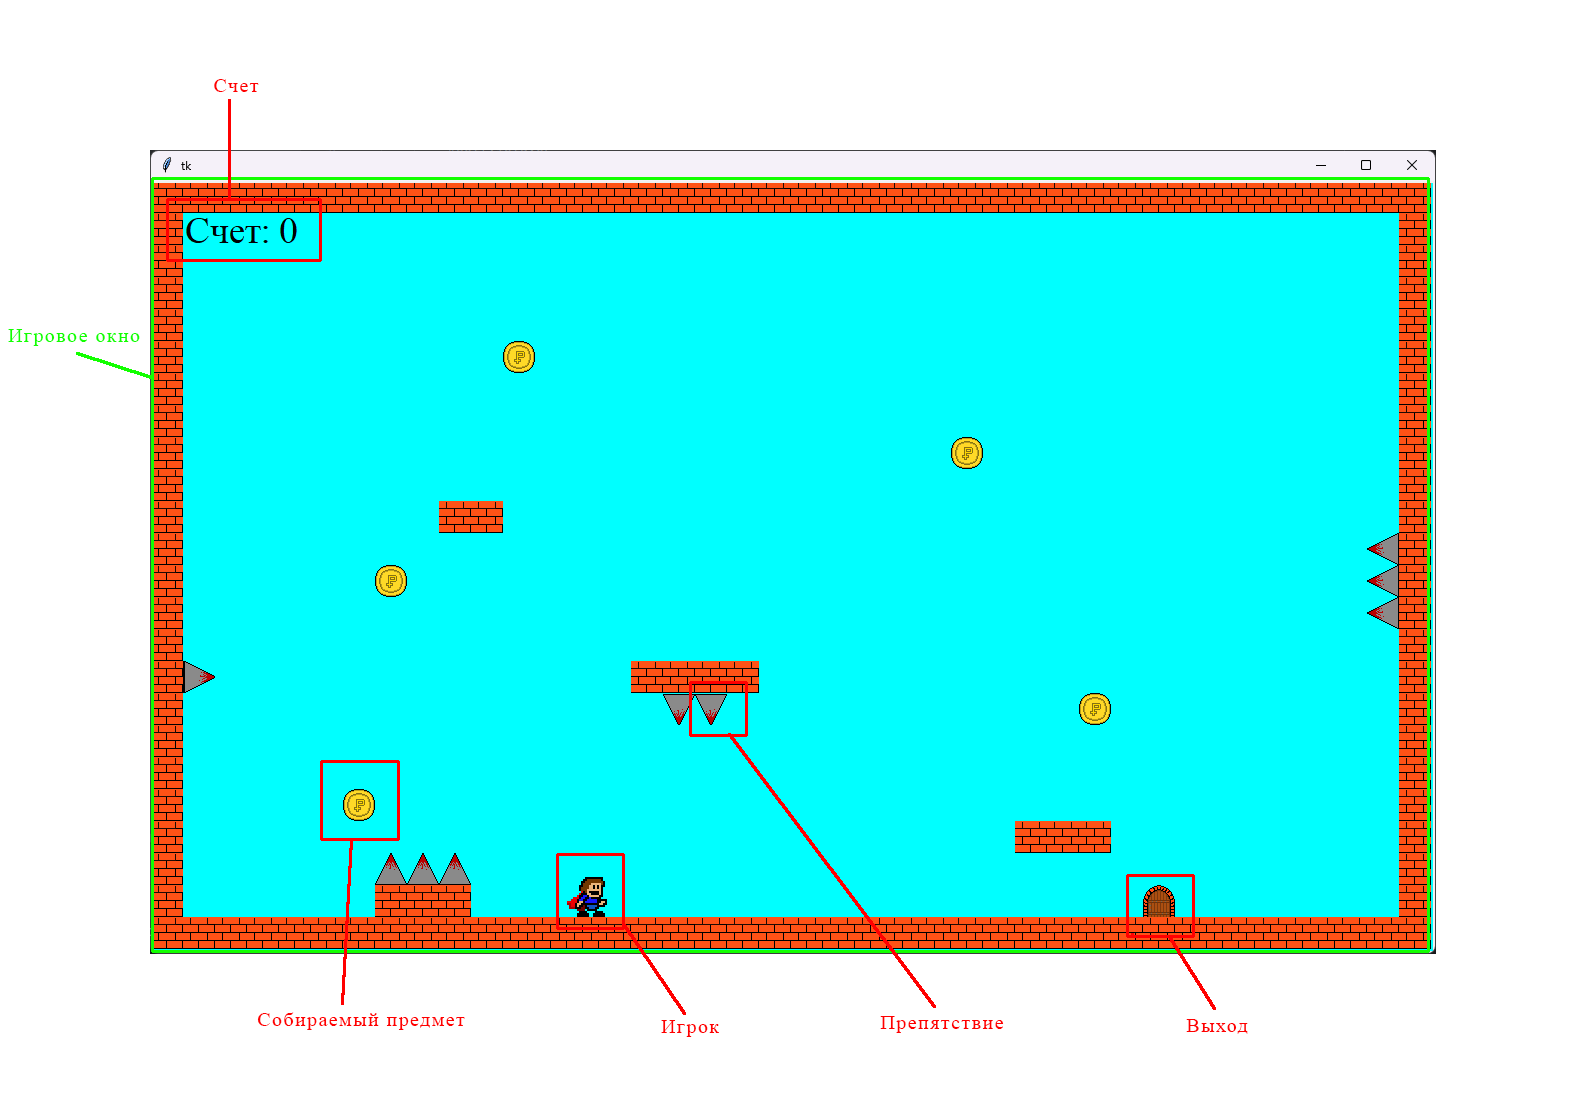
\includegraphics[width=1\linewidth]{templ}
\caption{Композиция шаблона игры}
\label{templ:image}
\end{figure}
%\vspace{-\figureaboveskip} % двойной отступ не нужен (можно использовать, если раздел заканчивается картинкой)

\subsection{Моделирование вариантов использования}

Для разрабатываемой игры была реализована модель, которая обеспечивает наглядное представление вариантов использования.

Она помогает в физической разработке и детальном анализе взаимосвязей объектов. При построении диаграммы вариантов использования применяется унифицированный язык визуального моделирования UML.

Диаграмма вариантов описывает функциональное назначение разрабатываемой системы. То есть это то, что система будет непосредственно делать в процессе своего функционирования. Она является исходным концептуальным представлением системы в процессе ее проектирования и разработки. Проектируемая система представляется в виде ряда прецедентов, предоставляемых системой актерам или сущностям, которые взаимодействуют с системой. Актером или действующим лицом является сущность, взаимодействующая с системой извне (например, человек, техническое устройство). Прецедент служит для описания набора действий, которые система предоставляет актеру.

На основании анализа предметной области в программе должны быть реализованы следующие прецеденты:
\subsubsection{Запуск игры}

При запуске игры выбирается ширина и высота окна, а также цвет фона, собирается уровень из массива, в котором указаны положения стен, предметов, выхода и самого игрока. Устанавливаются клавиши управления. Инициализируются все начальные значения переменных игры, загружаются изображения. Запускаются анимации для объектов.

\subsubsection{Прохождение уровня}

Игрок перемещается по карте двигаясь влево, вправо и прыгая. Игрок должен собрать все монеты и избегать препятствий, что бы пройти уровень. При передвижении влево и вправо, проигрываются соответствующие анимации. Что бы собрать все монеты игрок должен правильно проложить маршрут и точно прыгать по платформам. После сбора всех монет открывается дверь выхода. Добравшись до него игрок заканчивает уровень. Если игрок касается препятствия он погибает и начинает игру сначала теряя весь прогресс.

\subsubsection{Создание уровня}

Для создания уровня пользователь должен создать массив используя ключевые символы. Где s -- шип направленный вниз, a -- шип направленный влево, d -- шип направленный вправо, w -- шип направленный вверх, + -- монета, e -- выход, * -- игрок, - -- платформа.
\begin{figure}[H]
	\begin{lstlisting}[language=Python]
		LEVEL = ["----------------------------------------",
				 "-ssssssssssssssssssssssssssssssssssssss-",
				 "-                                      -",
				 "-                                      -",
				 "-                                      -",
			 	 "-          +                           -",
			     "-                                      -",
				 "-                                      -",
				 "-                        +             -",
				 "-                                      -",
				 "-        --                            -",
				 "-                                     a-",
				 "-      +                              a-",
				 "-                                     a-",
				 "-                                      -",
				 "-d             ----                    -",
				 "-               ss           +         -",
				 "-                                      -",
				 "-                                      -",
				 "-     +      *                         -",
				 "-                          ---         -",
				 "-      www                             -",
				 "-      ---                     e       -",
				 "----------------------------------------"]
	\end{lstlisting}  
	\caption{Пример массива уровня}
	\label{unitUser:image}
\end{figure}

\subsubsection{Отображение окна с результатом}

После прохождения уровня игрок получает сообщение с поздравлением и видит количество набранных им очков. Если игрок касается препятствие и проигрывает, он получается сообщение о поражении и так же видит количество набранных очков.

\subsection{Требования к оформлению документации}

Разработка программной документации и программного изделия должна производиться согласно ГОСТ 19.102-77 и ГОСТ 34.601-90. Единая система программной документации.
